\documentclass[tikz,border=0pt,crop=true]{standalone}

\usepackage{tikz} % Allows creation of tikz pictures
\usepackage{varwidth}
\usetikzlibrary{arrows,shapes}

\begin{document}
    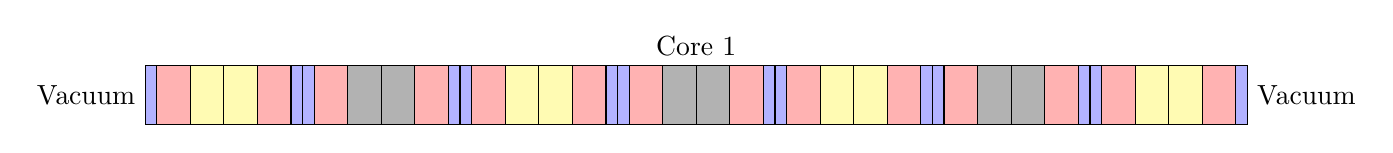
\begin{tikzpicture}[scale=1.0, every node/.style={scale=1}]
        % Draw the water cells
        \foreach \x in {0.0, 1.8533333, 2.0, 3.8533333, 4.0, 5.8533333, 6.0, 7.8533333, 8.0, 9.8533333, 10.0, 11.8533333, 12.0, 13.8533333}
        \filldraw[xshift=\x cm,fill=blue!30!white,draw=black] (0,0) 
        rectangle (0.14666667,.75);
        % Draw the uo2-1 cells
        \foreach \x in {0.1466667, 1.4266667, 2.1466667, 3.4266667, 4.1466667, 5.4266667, 6.1466667, 7.4266667, 8.1466667, 9.4266667, 10.1466667, 11.4266667, 12.1466667, 13.4266667}
        \filldraw[xshift=\x cm,fill=red!30!white,draw=black] (0,0) 
        rectangle (0.42666667,.75);
        % Draw the uo2-2 cells
        \foreach \x in {0.5733333, 1.0, 4.5733333, 5.0, 8.5733333, 9.0, 12.5733333, 13.0}
        \filldraw[xshift=\x cm,fill=yellow!30!white,draw=black] (0,0) 
        rectangle (0.42666667,.75);
        % Draw the uo2-Gd cells
        \foreach \x in {2.5733333, 3.0, 6.5733333, 7.0, 10.5733333, 11.0}
        \filldraw[xshift=\x cm,fill=black!30!white,draw=black] (0,0) 
        rectangle (0.42666667,.75);
        \draw (7,0.75) node[above] {Core 1};%
        \draw (14,0.375) node[right] {Vacuum};%
        \draw (0,0.375) node[left] {Vacuum};%
    \end{tikzpicture}
\end{document}
